\q{19}{Linear Regret-ssion} \\

We are interested in seeing how the Per Capita Income was related with Infant Mortality rate for various countries in the early 1950s. The data is encapsulated in a table named {\tt countries}, whose first few rows are shown below: 

\begin{center}
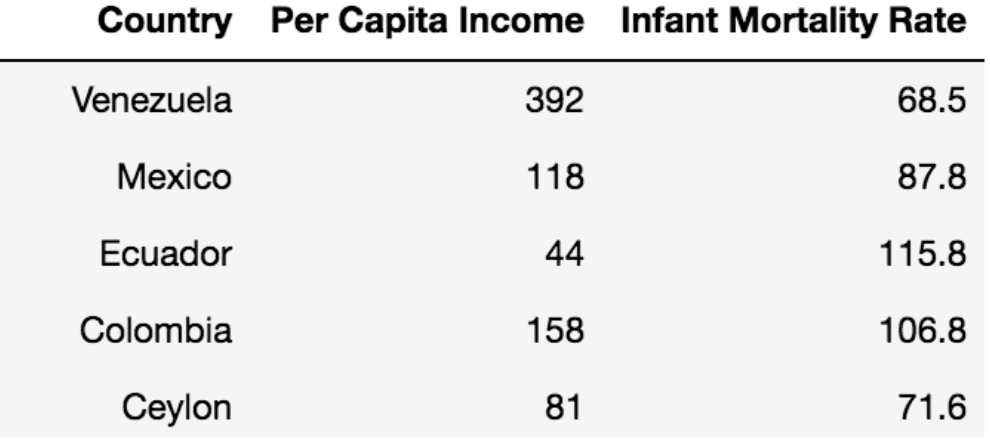
\includegraphics[scale=0.6]{regtable.png}
\end{center}

We are interested in looking at the relationship between Per Capita Income and Infant Mortality Rate. We plot two lines that we will use to predict infant mortality rate in a country (on average), given a per capita income. One is the regression line, and one is the constant line at the average of infant mortality rate. 

\begin{center}
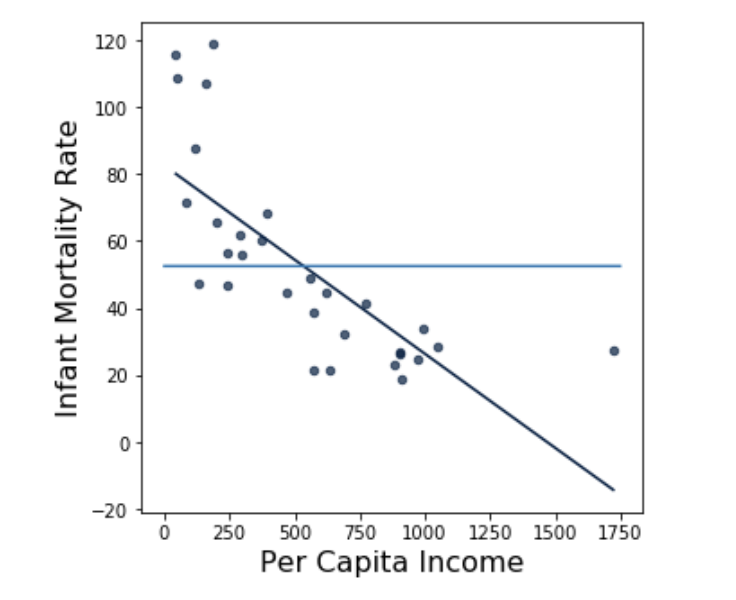
\includegraphics[scale=0.8]{regavg.png}
\end{center}

Here are some relevant lines of code and their outputs. Assume all of the functions below (descriptions of which appear on your study guide) are defined already. 

\begin{center}
 \begin{tabular}{||c c ||} 
 \hline
 Expression & Output\\ [0.5ex] 
 \hline\hline
 {\tt correlation(countries, 1, 2)} & -.74 \\ 
 \hline
 {\tt np.mean(countries.column(1))} & 534.1\\
 \hline
 {\tt np.mean(countries.column(2))} & 52.5\\
 \hline
 {\tt np.std(countries.column(1))} & 384.8\\
 \hline
 {\tt np.std(fitted\_values(countries, 1, 2))} & 21.6 \\ [1ex] 
 \hline
\end{tabular}
\end{center}


\begin{enumerate}

\subq{4} If possible, calculate the slope of the regression line in the plot above. Show your work with arithmetic. Please \textbf{do not} write any Python expressions. Box your final answer, which you may leave unsimplified. If it is not possible, explain why not. 
\\ \\ \\ \\ \\ \\ \\
\solution{Slope is r times the SD of y over SD of x. We have everything but SD of y. But, we can calculate that using the fact that we have the SD of the fitted values. The SD of the y is then $21.6 / .74$. We can then calculate for the slope using $r * \frac{SD(Y)}{SD(X)}$
}

\subq{2} At what value of per capita income would we predict the infant mortality rate to be 0 given the regression line on the previous page? 
\begin{itemize}[label=\bubble]
\item 0
\item 52.5
\item 80
\item 534.1
\item 1500
\item None of the above
\end{itemize} 
\solution{
	Option 5 -- based on graph
}



\subq{2} At what value of per capita income would we predict the infant mortality rate to be 0 given the average line on the previous page? 
\begin{itemize}[label=\bubble]
\item 0
\item 52.5
\item 80
\item 534.1
\item 1500
\item None of the above
\end{itemize} 
\solution{
	Option 6 -- based on graph 
} \\

\subq{3} Assume the RMSE (root mean squared error) of the regression line is 19.3. If possible, calculate the RMSE of the constant line representing the average of the infant mortality rate on this data. Show your work with arithmetic. Please \textbf{do not} write any Python expressions. Box your final answer, which you may leave unsimplified. If it is not possible, explain why not. \\ \\ \\ \\ \\ \\ \\
\solution{
The RMSE of the average line is actually just the SD of Infant Mortality Rate. We calculate that in Part a as $21.6 / .74$. 
}

\subq{3} If possible, fill in the blank with a mathematical expression. Box your final answer, which you may leave unsimplified. If it is not possible, explain why not. 
\\ \\ 
We use our regression line to estimate infant mortality rate using per capita income. At-least 88.9\% of our predictions of infant mortality rate will be correct within plus or minus \underline{\hspace{3cm}} units.
\solution{We notice that at least 88.9\% points us to three SDs both ways can be answered using Chebyshev's. We are trying to quantify the error, which is the residuals. So, we look at 3 SDs of the residuals both ways. We need to calculate the standard deviation of the residuals, which is $\sqrt{1-(-.74^2} * SD(Y)$. We calculated SD(Y) above, so our final answer is $3 * \sqrt{1 - .74**2} * 21.6 / .74$}

\\ \\
We move our attention to only the regression line and we would like to determine whether or not linear regression was a good idea to begin with. We show the regression line plotted on the scatter plot below again for convenience. \\
\begin{center}
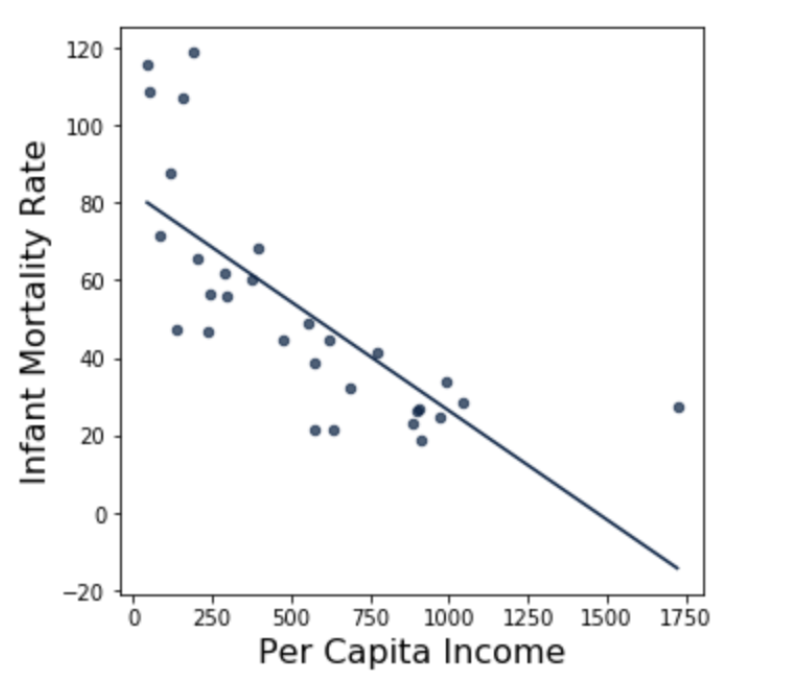
\includegraphics[scale=0.6]{regline.png}
\end{center} \\ \\
\subq{2} Which of the following plots is the best approximation to the residual plot, along with the line y=0?
\begin{multicols}{3}
\begin{itemize}[label=\bubble]
\item 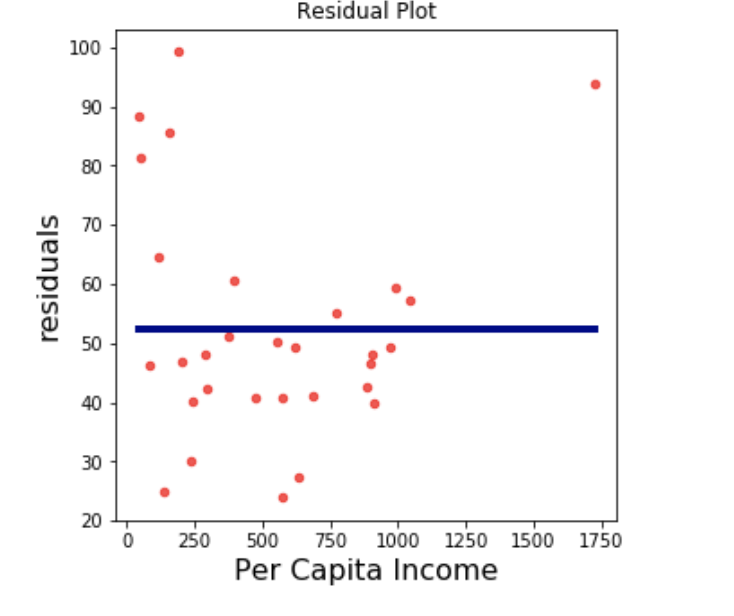
\includegraphics[scale=0.4]{resid2.png}
\item 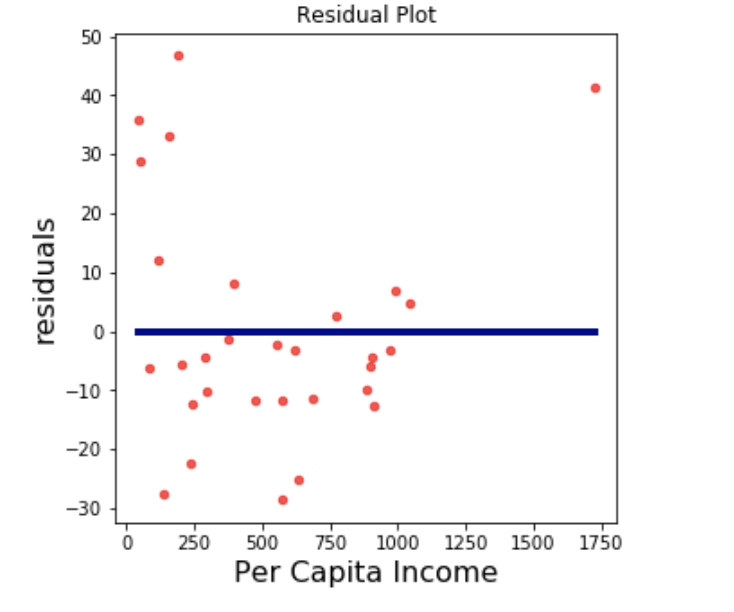
\includegraphics[scale=0.4]{resid1.png}
\item 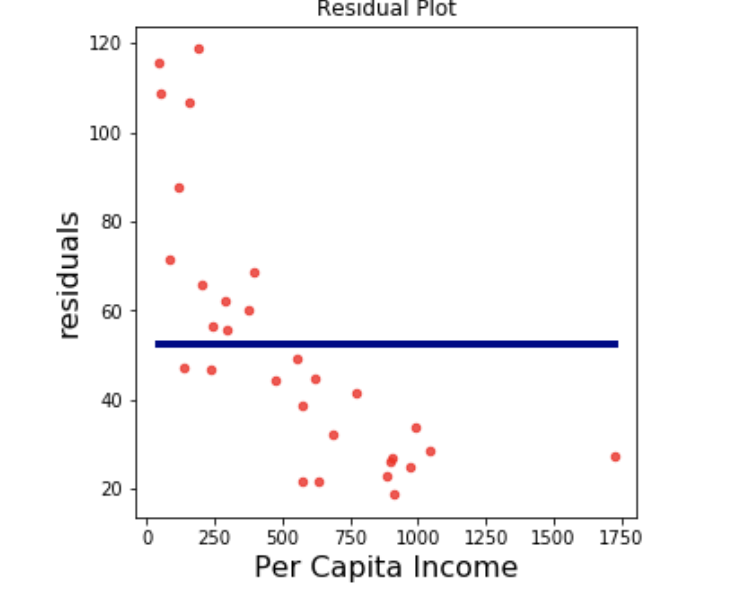
\includegraphics[scale=0.4]{resid3.png}
\end{itemize} 
\end{multicols}
\\ 
\solution{
	Option 2
}
\vfill

\subq{1} What is the approximate average value of the residuals? 
\begin{itemize}[label=\bubble]
\item -10
\item 0
\item 52.5
\item 534.1
\item Need more information
\end{itemize} 
\\ 
\solution{
	Option 2 -- Average of the residuals is always 0. 
}
\vfill
\subq{2} Based on the information above, select the most appropriate statement below. 
\begin{itemize}[label=\bubble]
\item Our residual plot shows no obvious pattern, so linear regression is a good fit for this data.
\item Our residual plot shows a definitive pattern, but based on our original plot, linear regression is still a good fit for this data.
\item Our residual plot shows a linearly decreasing trend, so linear regression is not a good fit for this data.
\item Our residual plot shows a definitive pattern, so linear regression is not a good fit for this data.
\item None of the above
\end{itemize} 
\\ 
\solution{
	Option 4 -- a pattern is present, but it is not decreasing linearly. It goes down, then comes back up. Since there is pattern in the residual plot, linear regression is not a good idea. 
}
\vfill



\end{enumerate}